\section{Overview and System Contract}
\label{sec:overview}

\subsection{From file operations to storage choices}

To read \code{src/parser.py}, a client resolves its name, obtains the
visible inode and data mappings, and fetches the requested bytes. An
overwrite stores new payload and updates the file's metadata under the
selected durability contract. \sys separates three decisions along this
path: which state the task sees, how immutable metadata is retrieved, and
how payloads are divided into storage units
(Table~\ref{tab:mechanism-choices}). On the object path, $g$ denotes client
block size, $B$ denotes backend erasure-coding block size, and $q$ denotes
the physical verification/read quantum.

\begin{table*}[t]
\centering
\small
\begin{tabularx}{\textwidth}{@{}p{3.0cm}YY@{}}
\toprule
Choice & Mechanism selected & Alternative retained\\
\midrule
View composition & Delta-based workspace: shared baseline plus private state & Ordinary volume with its own namespace and mappings\\
Immutable metadata & Packed Metadata: indexed records in bounded object-resident pages & Native catalog or KV representation\\
Object granularity & Configured client block size $g$; optional compatible backend $B/q$ choices & Fixed client geometry and backend default layout\\
\bottomrule
\end{tabularx}
\caption{Independent design decisions. A deployment selects mechanisms for
their own costs and contracts. Current mount paths support specific
combinations; this table is not a claim of eight interchangeable runtime modes.}
\label{tab:mechanism-choices}
\end{table*}

Each decision has its own input. A workspace binds a shared version and
resolves private changes against it; its lookup rules do not prescribe
the lower's metadata format. A packed reader obtains immutable records
from indexed pages and can also serve a read-only consumer. An ordinary
volume uses the object-data path without a shared baseline. When multiple
tasks reuse a stable environment, composing workspaces with a packed
baseline shares its representation while retaining private changes.

\subsection{Pinning state and isolating changes}

Let $S$ identify a shared immutable baseline and $\Delta_i$ the private
writable state of workspace $i$. Its view is
\begin{equation}
  W_i = \operatorname{Resolve}(S,\Delta_i).
\end{equation}
Workspace creation pins $S$ so that subsequent lower queries refer to the
same version. The baseline exposes name, attribute, and data-location
queries through either a sealed native layer or a packed manifest.
It can cover a selected subtree without freezing an entire source volume.
Following a mutable latest pointer on each lookup would not preserve
this fixed starting state.

Resolution checks private names, attributes, deletion state, and data
mappings before consulting $S$. A deletion marker suppresses an inherited
entry; absence of an upper record allows inheritance when no other rule
blocks it. Newly written payload bytes reside in separately referenced
objects. Thus an edit changes the workspace's records and references
without modifying the shared baseline.

The isolation invariant is view-local mutation: an operation in $W_i$
leaves $S$ and another workspace's private state unchanged. Concurrent
operations within one workspace must still preserve its namespace and
data invariants. Process isolation, network restrictions, and merging
independent edits require runtime or application protocols beyond this
file-view contract.

\subsection{Reading, writing, and publishing}

Figure~\ref{fig:overview} follows state references through the metadata and
object paths. For an inherited read, the chosen lower reader returns
metadata and resolves data locators to payload ranges. With a packed
lower, workspaces can reuse a fetched baseline page. If one workspace
overwrites the file, its private mapping refers to new upper bytes while
another workspace can continue to read $S$. The object's persisted layout
determines how the backend serves those bytes.

\begin{figure}[!t]
\centering
% Editable SVG with live text; regenerate with tools/draw_architecture_editable.py.
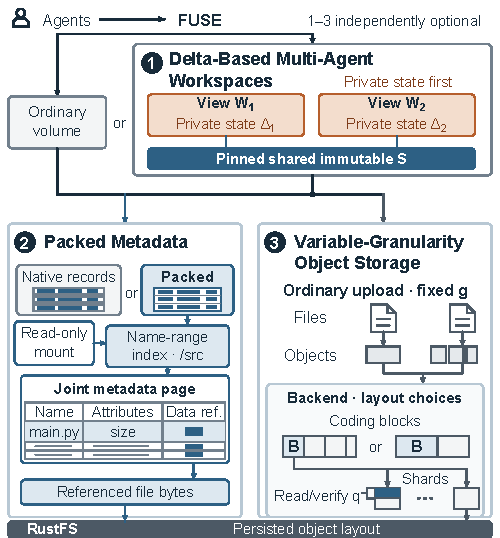
\includegraphics[width=\columnwidth]{figures/system-architecture-editable.pdf}

\caption{Three optional, composable mechanisms.
The metadata example stores file bytes separately.
In ordinary uploads, each raw block forms an object after applicable
compression/framing. Matching $U_1/O_p$ ports use separate upload contracts.
Dashed $B$ hints are optional; backends persist effective layouts.
Integration limits appear in Section~\ref{sec:implementation}.}
\label{fig:overview}
\end{figure}

Writes introduce two distinct visibility boundaries. A dirty buffer can
serve this client's reads before its bytes are remotely durable.
Publishing a recoverable immutable version requires its referenced
objects to satisfy the selected persistence contract and its metadata
to be validated. Private namespace state alone does not establish that
boundary, and a local read returning new bytes does not establish it
either.

Publication also creates a lifetime obligation: workspace and reader
ownership must retain referenced metadata and payloads until they can be
reclaimed. Backend layout selection can change how an object is encoded
and read while preserving its logical identity and contents. Readers of
an existing version continue to interpret each object using its persisted
layout.

A published file version may contain application checkpoints; restoring
process memory, open handles, and execution state remains the runtime's
responsibility. The next sections develop workspace resolution, immutable
metadata access, and object formation. Section~\ref{sec:implementation}
identifies their current mount and recovery paths.
